\section{TỔNG QUAN}
\hspace*{1cm} Quá trình đô thị hóa đang diễn ra mạnh mẽ tại Việt Nam, đặc biệt là ở các thành phố lớn như Thành phố Hồ Chí Minh (TPHCM) và Hà Nội. Theo dữ liệu của Tổng cục Thống kê, tỷ lệ đô thị hóa của Việt Nam đã đạt 42\% vào đầu năm 2023, trong đó số liệu TPHCM, Hà Nội và Đà Nẵng lần lượt là 77.7\%, 49.05\% và 87.45\% \cite{tyledothihoa}. Quá trình đô thị hóa dẫn đến sự gia tăng dân số đô thị và nhu cầu về nhà ở. Tuy nhiên, quỹ đất đô thị hạn chế khiến giá nhà ở đô thị ngày càng cao, vượt quá khả năng chi trả của nhiều người. Do đó, nhà trọ trở thành một hình thức nhà ở phổ biến tại các thành phố lớn.
\begin{figure}[H]
    \centering
    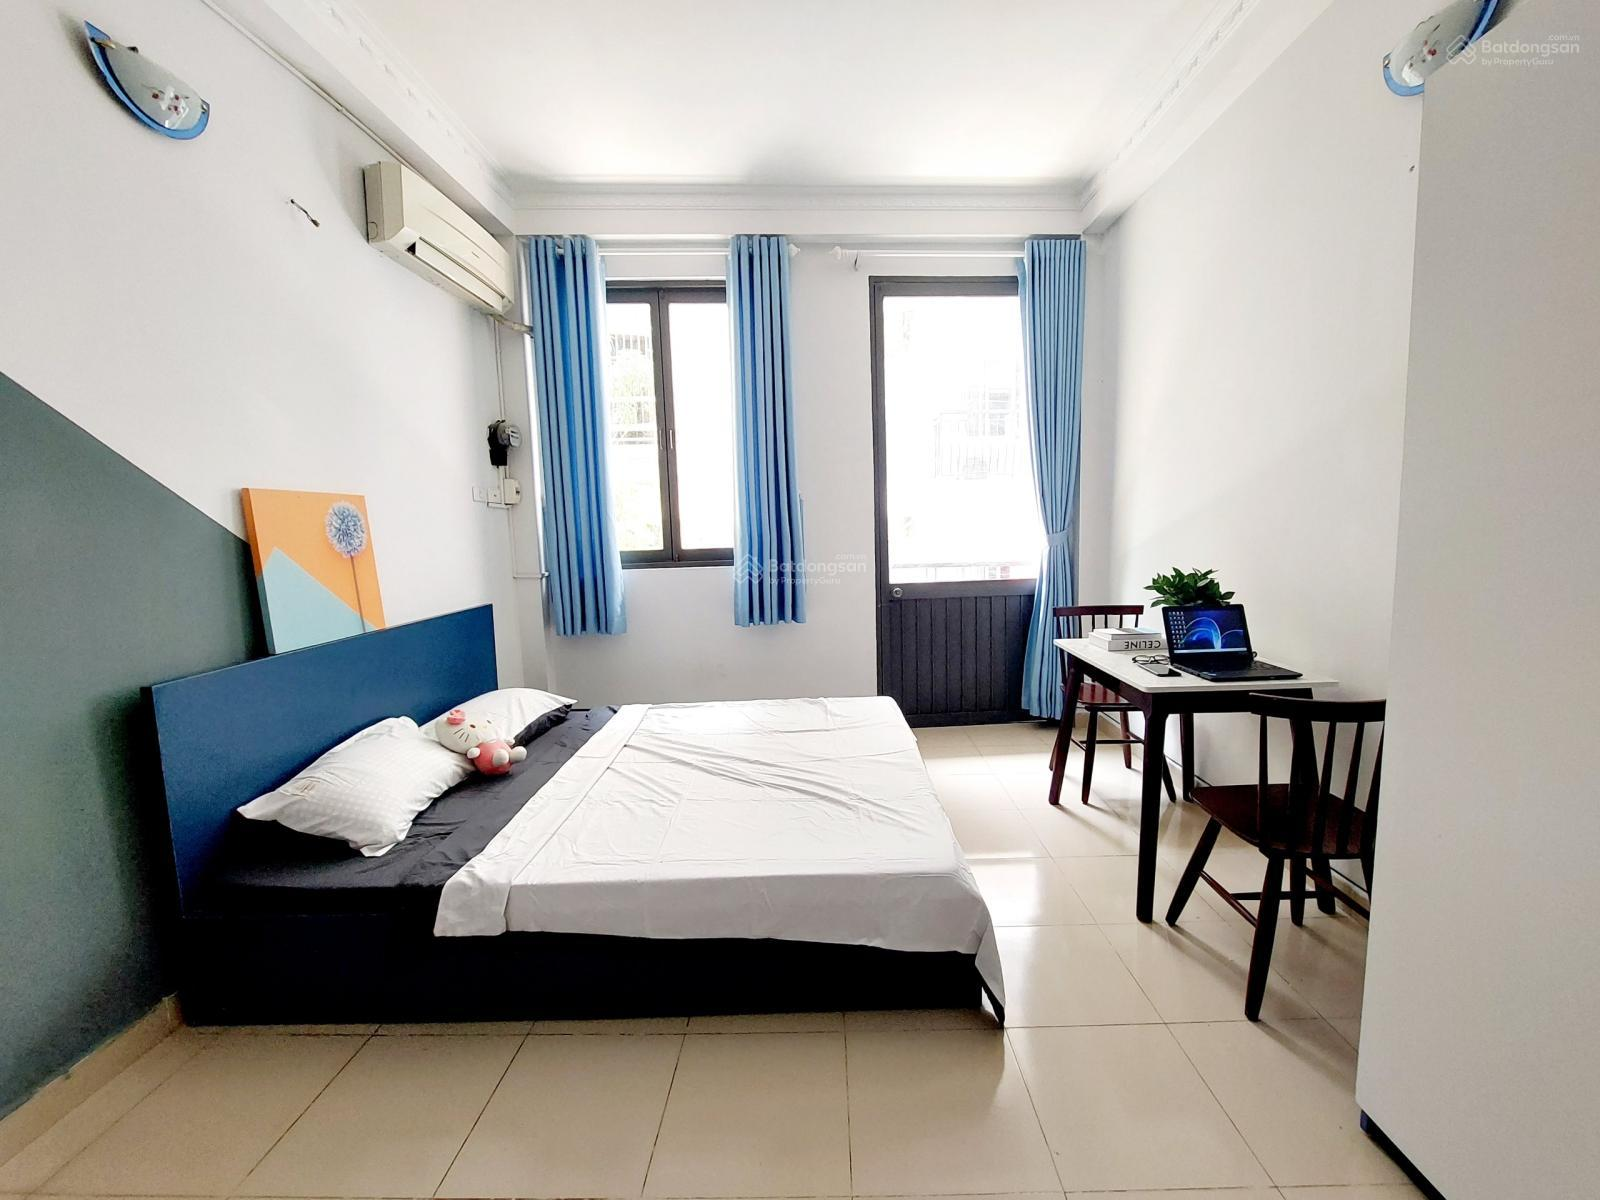
\includegraphics[width=0.7\textwidth]{Images/Overview/PhongTro.jpg}
    \caption{Một phòng trọ cho thuê tại phường Đa Kao, Quận 1, TP.HCM}
\end{figure}
\begin{figure}[H]
    \centering
    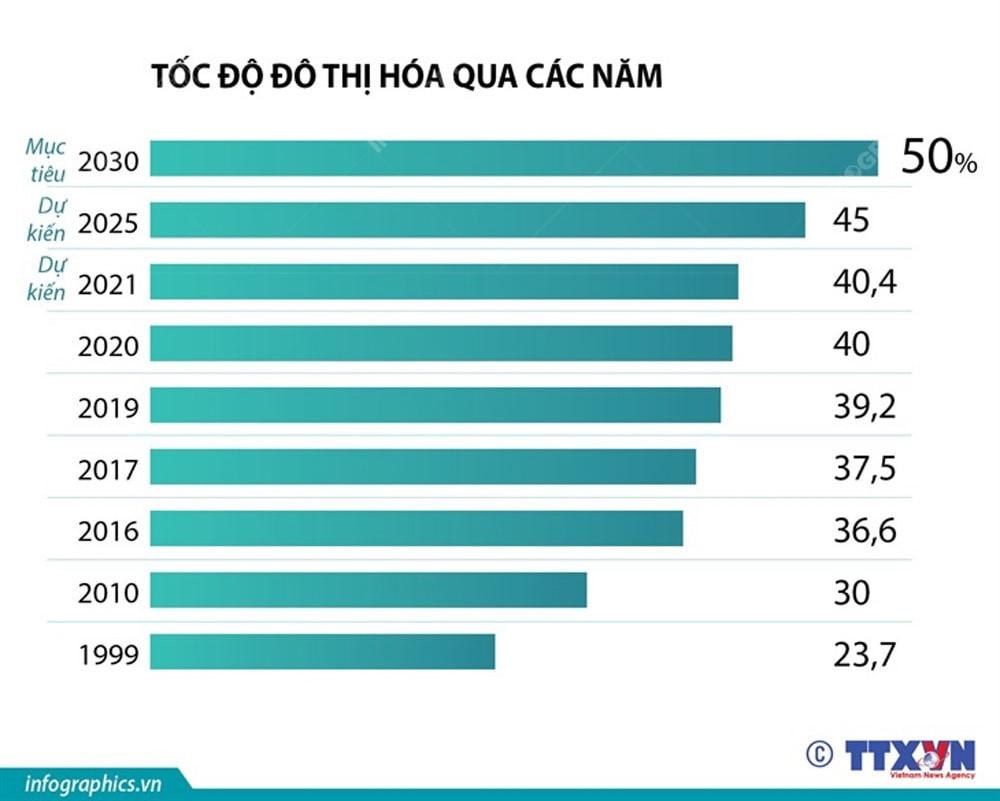
\includegraphics[width=0.6\textwidth]{Images/Overview/TocDoDoThiHoa.jpg}
    \caption{Tốc độ đô thị hóa tại Việt Nam trong 30 năm qua (Nguồn: TTXVN)}
\end{figure}
\begin{figure}[H]
    \centering
    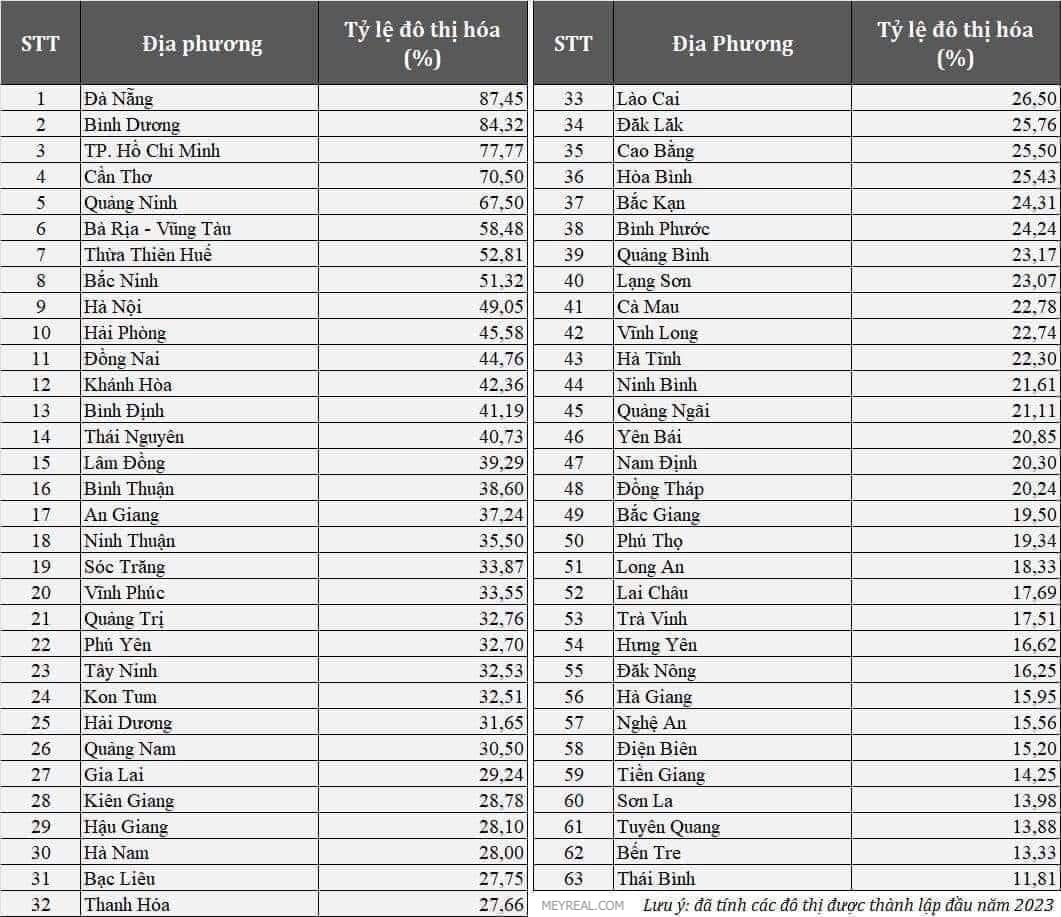
\includegraphics[width=0.95\textwidth]{Images/Overview/TyLeDoThiHoa.jpg}
    \caption{Tỷ lệ đô thị hóa tại các tỉnh thành ở Việt Nam đầu năm 2023 (Nguồn: Kavi Group)}
\end{figure}
\hspace*{1cm} Dựa trên thông tin từ Báo Phụ Nữ \cite{phunu} và Kinh Tế Môi Trường \cite{ktmt}, năm 2022 đã chứng kiến sự phát triển vượt bậc của thị trường nhà trọ tại Việt Nam. Cụ thể, sau một quý I/2022 với mức tăng trưởng ấn tượng, quý II/2022 tiếp tục ghi nhận sự tăng nhẹ trong nguồn cung phòng trọ với mức tăng gần 2\%. Tại TPHCM và tỉnh Bình Dương, mức tăng lần lượt đạt 4,5\% và 12,8\%. Trong khi đó, nguồn cung phòng trọ tại Hà Nội và Đà Nẵng lại giảm lần lượt với tỉ lệ là 10\% và 5,5\%. Nhu cầu thuê nhà trọ, đặc biệt là tại các khu vực lân cận các trường đại học ở TPHCM và Hà Nội, đã tăng mạnh trong năm 2022. Điều này là do quá trình nhập học của năm 2022 đã trở lại bình thường sau một thời gian dài bị ảnh hưởng bởi dịch COVID-19, và một lượng lớn sinh viên mới sẽ cần tìm chỗ ở để phục vụ quá trình học tập tại các thành phố lớn.ẽ có nhu cầu tìm chỗ ở phục vụ quá trình học tập tại các thành phố lớn.
Nhu cầu thuê trọ của các đối tượng cư dân đô thị rất đa dạng, bao gồm:
\begin{itemize}
    \item \textit{Sinh viên:} Sinh viên là đối tượng có nhu cầu thuê trọ cao nhất tại các thành phố lớn. Theo thống kê của Bộ Giáo dục và Đào tạo, tính đến năm 2022, cả nước có khoảng 10 triệu sinh viên, trong đó có khoảng 4 triệu sinh viên đang theo học tại các trường đại học, cao đẳng ở TPHCM và Hà Nội.
    \item \textit{Công nhân:} Công nhân cũng là một đối tượng có nhu cầu thuê trọ cao tại các thành phố lớn. Theo thống kê của Tổng cục Thống kê, tính đến năm 2022, cả nước có khoảng 15 triệu lao động làm việc trong các khu công nghiệp, trong đó có khoảng 5 triệu lao động đang làm việc tại các khu công nghiệp ở TPHCM và Hà Nội.
    \item \textit{Người dân:} Ngoài sinh viên và công nhân, còn có một số đối tượng khác cũng có nhu cầu thuê trọ, chẳng hạn như người lao động tự do, người về hưu,...
\end{itemize}
Trong thời đại số hóa, việc sử dụng điện thoại thông minh để tìm kiếm, đăng tin và quản lý nhà trọ đã trở thành một phần không thể thiếu và tiện lợi. smartphone, với sự đa dạng về chức năng và ứng dụng, đã trở thành thiết bị di động phổ biến nhất hiện nay. Theo VTV, vào năm 2022, số lượng người dùng điện thoại thông minh trên toàn cầu ước tính đạt 6,6 tỷ người, tăng 4,9\% hàng năm \cite{smartphone2022}. Tại Việt Nam, theo Chiến lược hạ tầng số quốc gia đến năm 2025, mục tiêu là 85\% người trưởng thành sẽ sở hữu điện thoại thông minh \cite{chienluoc}. Đại diện Cục Viễn thông (Bộ Thông tin và Truyền thông) cho biết, vào cuối năm 2021, Việt Nam đã có 91,3 triệu thuê bao điện thoại thông minh \cite{vnsmartphone}.
\begin{figure}[h]
    \centering
    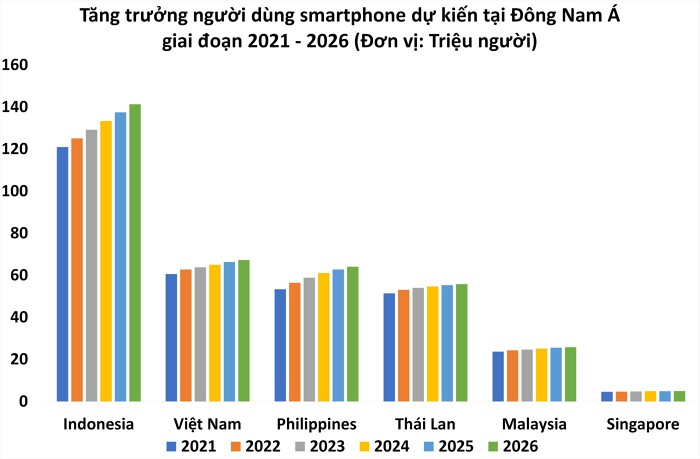
\includegraphics[width=1\textwidth]{Images/Overview/TangTruongSmartphone.jpg}
    \caption{Tăng trưởng người dùng smartphone tại Đông Nam Á giai đoạn 2021 - 2026 (Nguồn: VietnamBiz)}
\end{figure}
Với sự phát triển của công nghệ thông tin, các chủ kinh doanh nhà trọ đã bắt đầu sử dụng các nền tảng mạng xã hội như Facebook, Zalo,... để quảng bá nhà trọ của mình. Tuy nhiên, cách thức quảng bá này vẫn còn tồn tại một số bất cập, cụ thể như sau:
\begin{itemize}
    \item \textit{Phạm vi tiếp cận hạn chế:} Các nền tảng mạng xã hội có lượng người dùng đông đảo, nhưng không phải tất cả những người dùng này đều có nhu cầu thuê nhà trọ. Do đó, việc quảng bá nhà trọ trên các nền tảng mạng xã hội sẽ khiến cho thông tin nhà trọ tiếp cận được với một số lượng người dùng hạn chế.
    \item \textit{Thông tin không được phân loại:} Thông tin nhà trọ được đăng tải trên các nền tảng mạng xã hội thường không được phân loại theo các tiêu chí như vị trí, giá cả, tiện ích,... Điều này khiến cho người thuê trọ khó có thể tìm kiếm được nhà trọ phù hợp với nhu cầu của mình. 
    \item \textit{Tính cạnh tranh cao:} Trên các nền tảng mạng xã hội, có rất nhiều thông tin nhà trọ được đăng tải. Điều này khiến cho thông tin nhà trọ của các chủ kinh doanh nhà trọ dễ bị \textit{"chìm"} và không được người thuê trọ chú ý.
\end{itemize}
Tương tự như trên, với sự phát triển của công nghệ thông tin, việc tìm kiếm nhà trọ đã trở nên dễ dàng hơn bao giờ hết. Tuy nhiên, bên cạnh những lợi ích, việc tìm kiếm nhà trọ qua các nền tảng công nghệ thông tin cũng tồn tại một số bất cập, cụ thể như sau:
\begin{itemize}
    \item \textit{Thiếu thông tin chính xác:} Thông tin nhà trọ được đăng tải trên các nền tảng công nghệ thông tin thường chỉ bao gồm những thông tin cơ bản như diện tích, giá cả, vị trí,... Điều này khiến cho người thuê trọ khó có thể đánh giá được chất lượng thực tế của nhà trọ. Ngoài ra, một số trường hợp chủ kinh doanh nhà trọ cố tình đăng tải thông tin nhà trọ không chính xác để thu hút khách hàng.
    \item \textit{Khó khăn để tìm kiếm nhà trọ phù hợp:} Các nền tảng công nghệ thông tin có lượng thông tin nhà trọ rất lớn, nhưng không được phân loại theo các tiêu chí như vị trí, giá cả, tiện ích,... Điều này khiến cho người thuê trọ khó có thể tìm kiếm được nhà trọ phù hợp với nhu cầu của mình.
    \item \textit{Tốn thời gian và công sức:} Để tìm được nhà trọ phù hợp, người thuê trọ thường phải mất nhiều thời gian để tìm kiếm thông tin trên các nền tảng công nghệ thông tin. Ngoài ra, người thuê trọ cũng phải gặp gỡ trực tiếp chủ kinh doanh nhà trọ để xem xét nhà trọ trước khi quyết định thuê.
\end{itemize}
Trước bối cảnh gia tăng nhu cầu về phòng trọ, sự phát triển của smartphone cũng như nhìn nhận ra những vấn đề mà người chủ trọ cũng như người thuê trọ có thể gặp phải trong việc đăng tải và tìm thuê nhà trọ, nhóm nghiên cứu muốn hướng đến một giải pháp tìm kiếm nhà trọ thông minh trên thiết bị di động, nhằm tạo ra sự tiện lợi và nhanh chóng trong việc kết nối giữa chủ trọ và người thuê.